We apply the mistake taxonomy from Table~\ref{tab:taxonomy} to all ten runs.
Problems where at least one of 8 samples is correct (pass8=True but pass1=False) are excluded, as they represent consistency failures rather than knowledge gaps.

\textbf{Error distributions.}
Table~\ref{tab:p4-errors} shows the distribution of mistake types across runs, counted over problems where all 8 samples failed (pass8=False).

\begin{table}[H]
\centering
\small
\begin{tabular}{lrrrrrr}
\toprule
\textbf{Run} & \textbf{No Ans.} & \textbf{Fmt Only} & \textbf{No Reas.} & \textbf{Arith.} & \textbf{Wrong Set.} & \textbf{Gibb.} \\
\midrule
Baseline & 273 (27.6\%) & 389 (39.3\%) & 0 & 110 (11.1\%) & 186 (18.8\%) & 32 (3.2\%) \\
\midrule
+ A & 127 (14.4\%) & 153 (17.4\%) & 0 & 173 (19.7\%) & 397 (45.1\%) & 30 (3.4\%) \\
+ B & 244 (25.2\%) & 304 (31.4\%) & 0 & 137 (14.1\%) & 254 (26.2\%) & 30 (3.1\%) \\
+ A+B & 171 (18.6\%) & 190 (20.7\%) & 0 & 177 (19.2\%) & 356 (38.7\%) & 26 (2.8\%) \\
\bottomrule
\end{tabular}
\caption{Mistake type distribution for problems where all 8 samples failed (pre-P3 runs). Percentages are within each run's failed set.}
\label{tab:p4-errors}
\end{table}

\textbf{Distribution shifts.}
Figure~\ref{fig:p4-error-dist} visualizes the error composition across runs.

\vspace{1em}
\noindent\begin{minipage}{\linewidth}
\centering
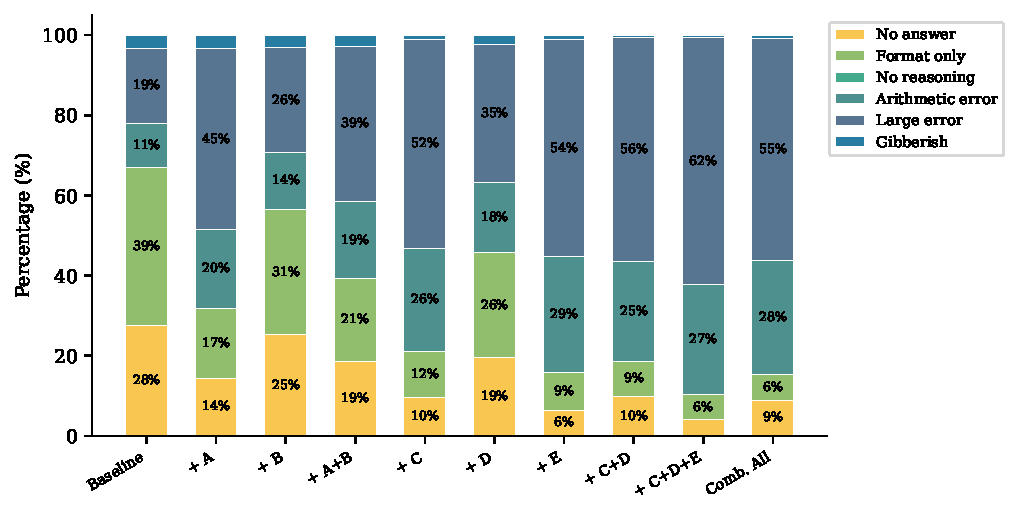
\includegraphics[width=\linewidth]{component/figures/p4/fig4_error_distribution.pdf}
\captionof{figure}{Error category composition (\%) across all runs. The shift from format-related failures (no answer, format only) toward reasoning failures (large error, arithmetic error) is visible across all reward additions.}
\label{fig:p4-error-dist}
\end{minipage}
\vspace{1em}

The dominant pattern across all reward additions is a shift from format-related failures (no answer, format only) toward content-related failures (large error, arithmetic error).
Reward A produces the largest shift: ``no answer'' drops from \pFourBaselineNoAnswer\% to \pFourSeparateANoAnswer\% ($-$13.1pp) and ``format only'' drops from \pFourBaselineFormatOnly\% to \pFourSeparateAFormatOnly\% ($-$21.9pp), while ``large error'' rises from \pFourBaselineLargeError\% to \pFourSeparateALargeError\% (+26.3pp).
This is expected---format compliance reward teaches the model to produce parseable answers, converting previously unparseable responses into formatted-but-wrong ones.
The shift reveals that many baseline ``format failures'' were masking underlying reasoning errors.

Reward B shows the same directional pattern but at smaller magnitude, consistent with its modest accuracy improvement.
